\newpage
\section{Parameter Identification and Validation}

Thus, the process model for $NO_x$ input and output dynamics is put into the regression form in equation
\ref{eqn::final_simplified_regression}. Least-squares cannot be directly applied to the above regression model as the
condition number of the resulting matrix is very high (order of $10^{18}$). This is due to the fact that individual
elements of the $\pmb phi_r$ vector are of significantly different order of magnitudes. This numerical issue can be
resolved by scaling the equation appropriately. It has also been verified that all the available data sets satisfy the weekly persistent excitation condition. Consider,
\begin{align*}
        y_r &= \pmb \phi_r^T \pmb \theta_{NO_x} + \varepsilon\\
        \text{Let, } \qquad W &= diag \bm{w_1, w_2, \hdots, w_8}\\
        \text{then, } \quad y_r &= \underbrace{\pmb \phi_r^T  W}_{\pmb \phi_rw}
                        \underbrace{ W^{-1} \pmb \theta_{NO_x}}_{\pmb \theta_{wNO_x}} + \varepsilon\\
        \implies y_r &= \pmb \phi_{rw} \pmb \theta_{w NO_x} + \varepsilon
\end{align*}
Thus, scaling the regressor in above fashion doesn't effect the model structure errors. The actual parameter vector $\pmb \theta_{NO_x}$ can be obtained by multiplying the scaling matrix to the estimate again.
\begin{align*}
        \hat{\pmb \theta}_{NO_x} &= W \hat{\pmb \theta}_{wNO_x}
\end{align*}
The elements of W are chosen such that the order of magnitude of each of the elements of $\pmb \phi_r$ are same as that of $\pmb y_r$.

From the available test data, we have the elements of scaling matrix:
\begin{table}[H]
        \centering
        \begin{tabular}{c c c c c c c c c c}
                $w_0$ & $w_1$  & $w_2$     & $w_3$     & $w_4$     & $w_5$     & $w_6$  & $w_7$ \\
                $1$   & $10^2$ & $10^{-3}$ & $10^{-1}$ & $10^{-4}$ & $10^{-2}$ & $10^2$ & $10^{4}$
        \end{tabular}
\end{table}

These weights are used for both parameter estimation using the least-squares and the recursive least-squares. The one-step ahead prediction error for RLS and the clustering of parameter vectors in 2-D space based on aging level are presented in the next section.

\newpage
\section{Cross validation results}

\subsection{Degreened Test Data}

\begin{figure}[H]
        \begin{minipage}{0.33\textwidth}
                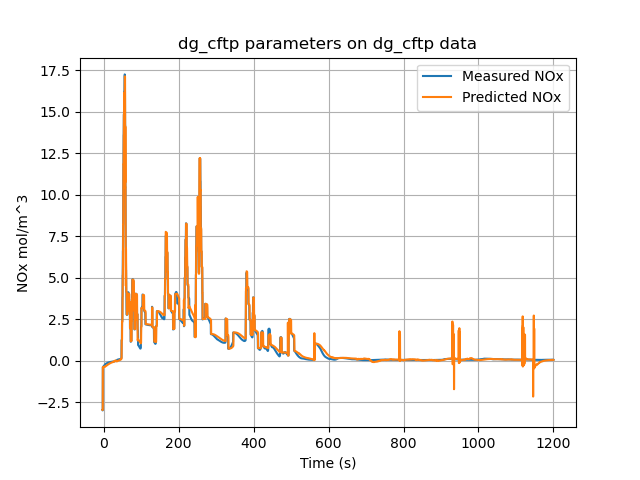
\includegraphics[width = \textwidth]{\froot/figs/figs_new_mdl/dg_cftp_dg_cftp.png}
        \end{minipage}
        \begin{minipage}{0.33\textwidth}
                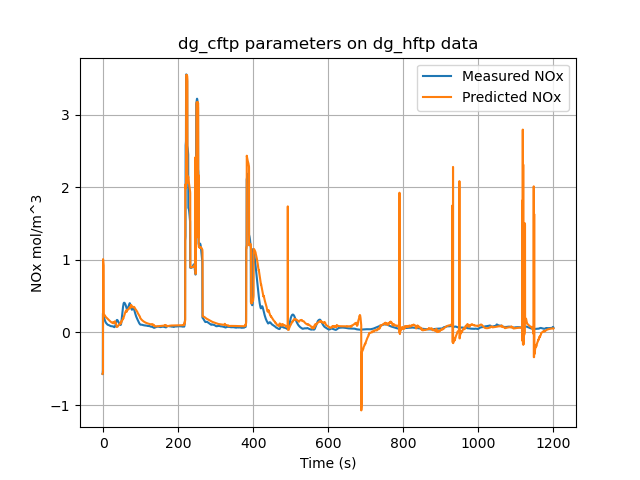
\includegraphics[width = \textwidth]{\froot/figs/figs_new_mdl/dg_cftp_dg_hftp.png}
        \end{minipage}
        \begin{minipage}{0.33\textwidth}
                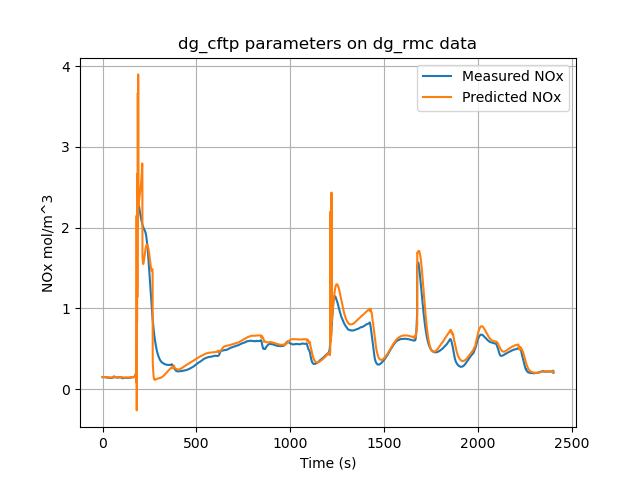
\includegraphics[width = \textwidth]{\froot/figs/figs_new_mdl/dg_cftp_dg_rmc.png}
        \end{minipage}
        \caption{Cross validation using dg$\_$cftp parameter estimates}
\end{figure}

\begin{figure}[H]
        \begin{minipage}{0.33\textwidth}
                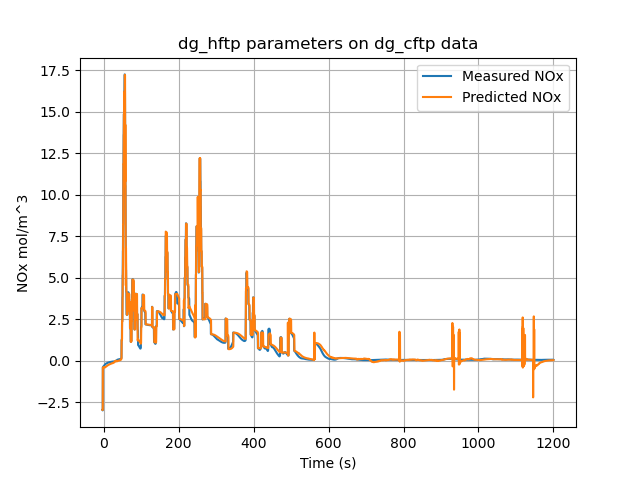
\includegraphics[width = \textwidth]{\froot/figs/figs_new_mdl/dg_hftp_dg_cftp.png}
        \end{minipage}
        \begin{minipage}{0.33\textwidth}
                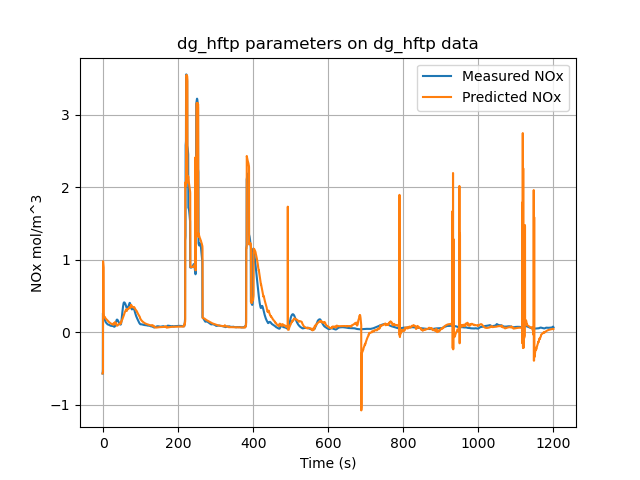
\includegraphics[width = \textwidth]{\froot/figs/figs_new_mdl/dg_hftp_dg_hftp.png}
        \end{minipage}
        \begin{minipage}{0.33\textwidth}
                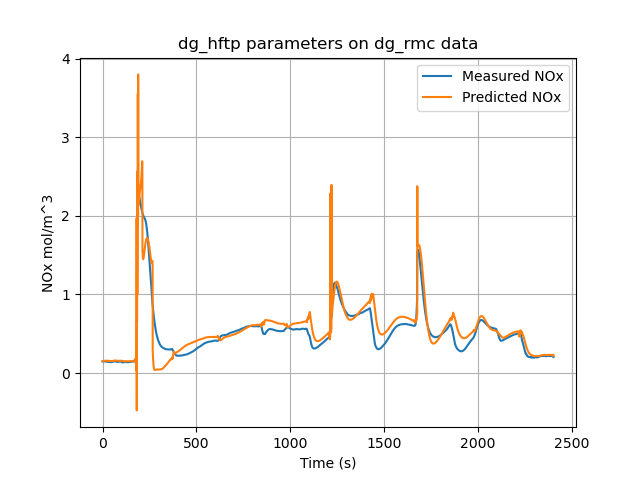
\includegraphics[width = \textwidth]{\froot/figs/figs_new_mdl/dg_hftp_dg_rmc.png}
        \end{minipage}
        \caption{Cross validation using dg$\_$hftp parameter estimates}
\end{figure}

\begin{figure}[H]
        \begin{minipage}{0.33\textwidth}
                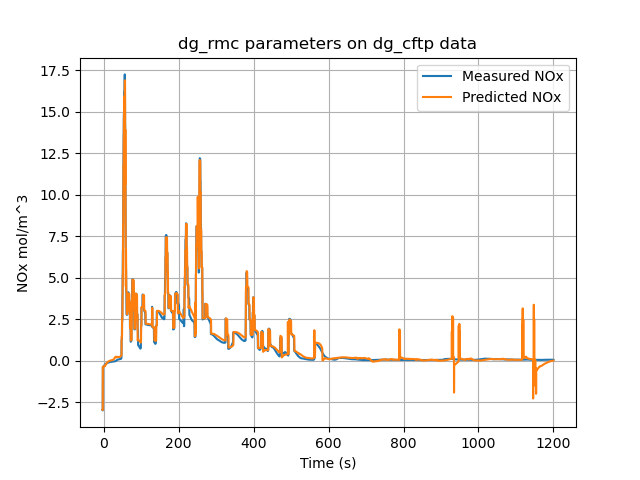
\includegraphics[width = \textwidth]{\froot/figs/figs_new_mdl/dg_rmc_dg_cftp.png}
        \end{minipage}
        \begin{minipage}{0.33\textwidth}
                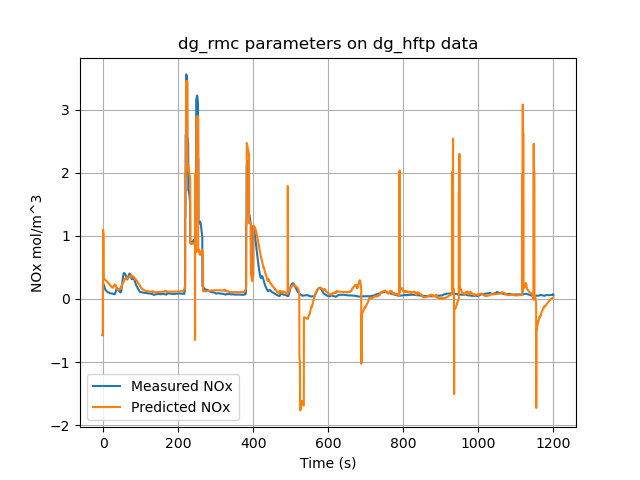
\includegraphics[width = \textwidth]{\froot/figs/figs_new_mdl/dg_rmc_dg_hftp.png}
        \end{minipage}
        \begin{minipage}{0.33\textwidth}
                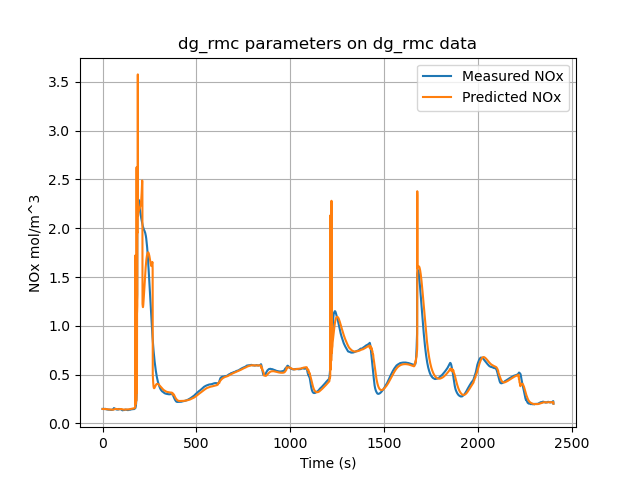
\includegraphics[width = \textwidth]{\froot/figs/figs_new_mdl/dg_rmc_dg_rmc.png}
        \end{minipage}
        \caption{Cross validation using dg$\_$rmc parameter estimates}
\end{figure}


\subsection{Aged Test Data}

\begin{figure}[H]
        \begin{minipage}{0.33\textwidth}
                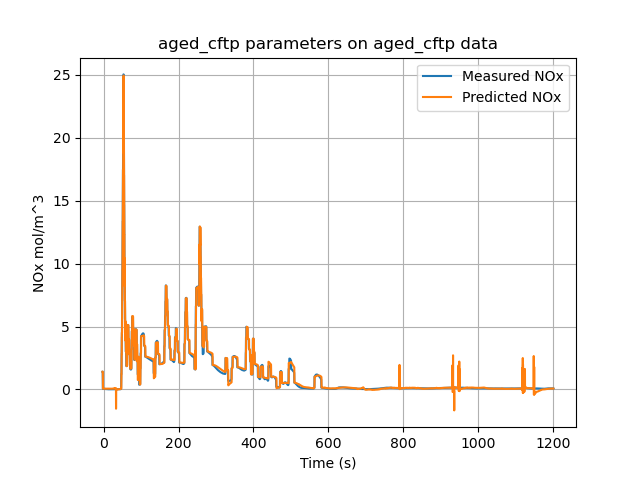
\includegraphics[width = \textwidth]{\froot/figs/figs_new_mdl/aged_cftp_aged_cftp.png}
        \end{minipage}
        \begin{minipage}{0.33\textwidth}
                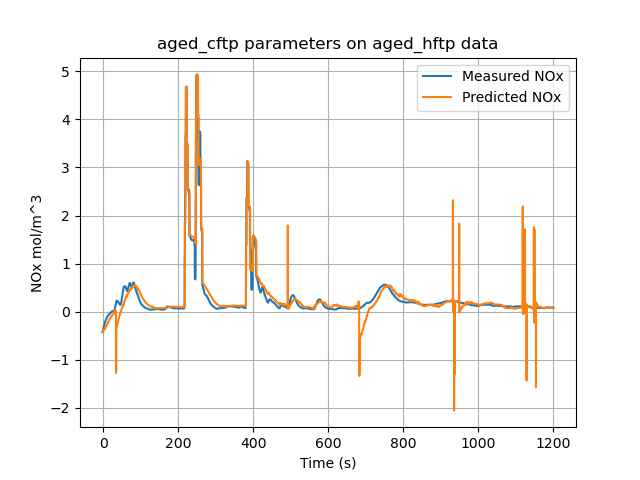
\includegraphics[width = \textwidth]{\froot/figs/figs_new_mdl/aged_cftp_aged_hftp.png}
        \end{minipage}
        \begin{minipage}{0.33\textwidth}
                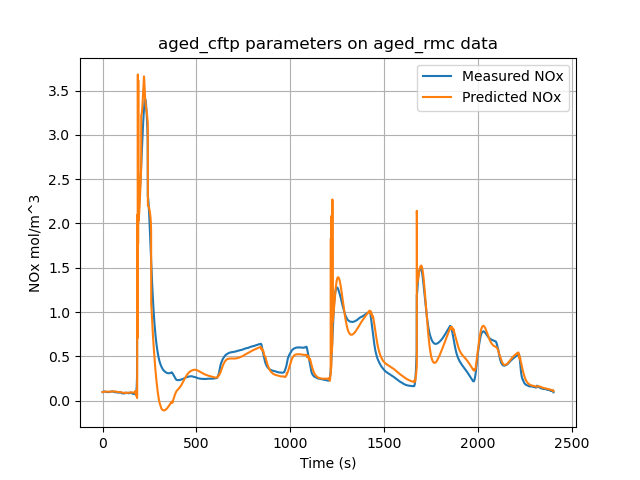
\includegraphics[width = \textwidth]{\froot/figs/figs_new_mdl/aged_cftp_aged_rmc.png}
        \end{minipage}
        \caption{Cross validation using aged$\_$cftp parameter estimates}
\end{figure}

\begin{figure}[H]
        \begin{minipage}{0.33\textwidth}
                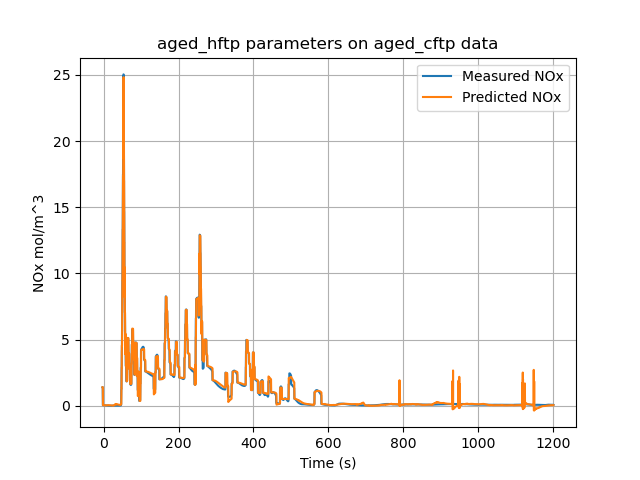
\includegraphics[width = \textwidth]{\froot/figs/figs_new_mdl/aged_hftp_aged_cftp.png}
        \end{minipage}
        \begin{minipage}{0.33\textwidth}
                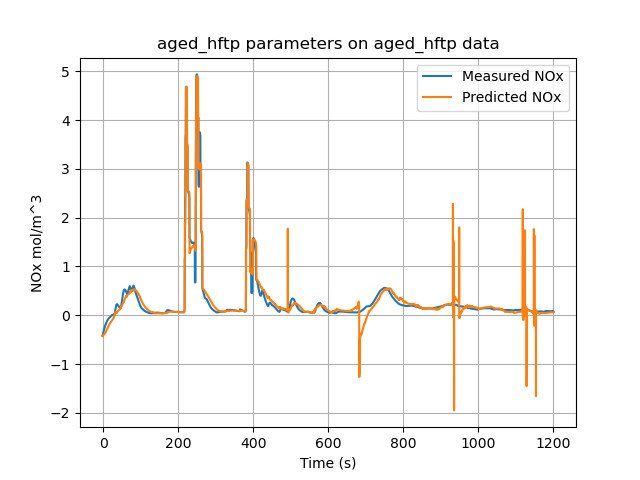
\includegraphics[width = \textwidth]{\froot/figs/figs_new_mdl/aged_hftp_aged_hftp.png}
        \end{minipage}
        \begin{minipage}{0.33\textwidth}
                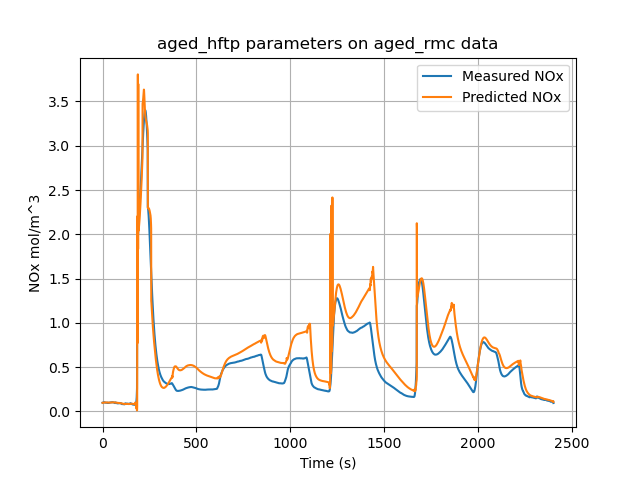
\includegraphics[width = \textwidth]{\froot/figs/figs_new_mdl/aged_hftp_aged_rmc.png}
        \end{minipage}
        \caption{Cross validation using aged$\_$hftp parameter estimates}
\end{figure}

\begin{figure}[H]
        \begin{minipage}{0.33\textwidth}
                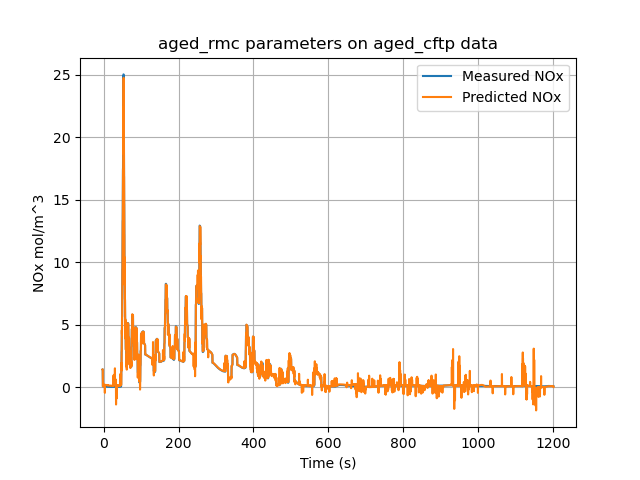
\includegraphics[width = \textwidth]{\froot/figs/figs_new_mdl/aged_rmc_aged_cftp.png}
        \end{minipage}
        \begin{minipage}{0.33\textwidth}
                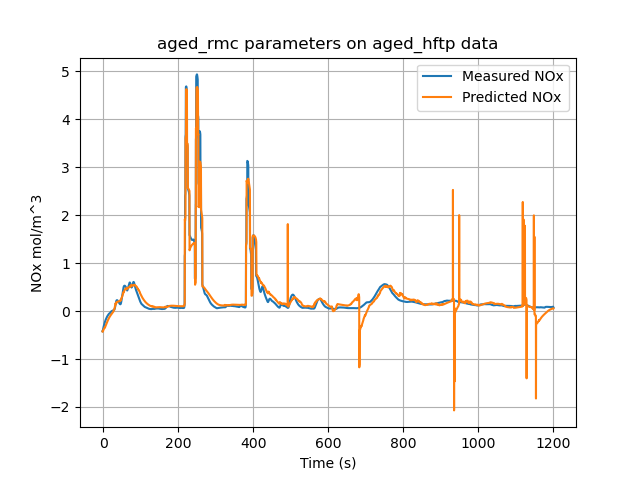
\includegraphics[width = \textwidth]{\froot/figs/figs_new_mdl/aged_rmc_aged_hftp.png}
        \end{minipage}
        \begin{minipage}{0.33\textwidth}
                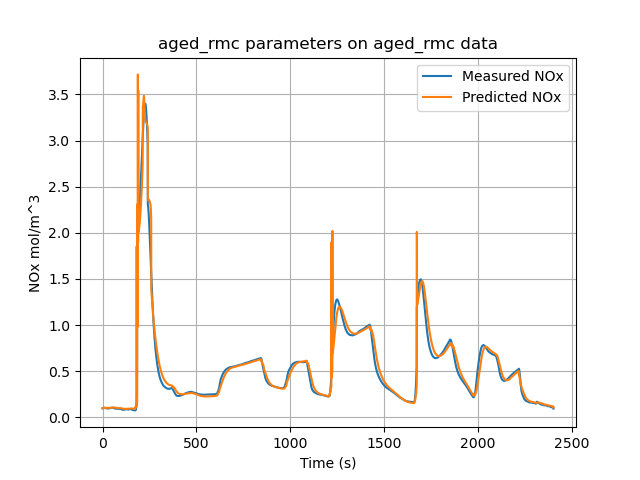
\includegraphics[width = \textwidth]{\froot/figs/figs_new_mdl/aged_rmc_aged_rmc.png}
        \end{minipage}
        \caption{Cross validation using aged$\_$rmc parameter estimates}
\end{figure}


\subsection{Comparing Aged and Degreened parameter estimates}

\begin{figure}[H]
        \begin{minipage}{0.33\textwidth}
                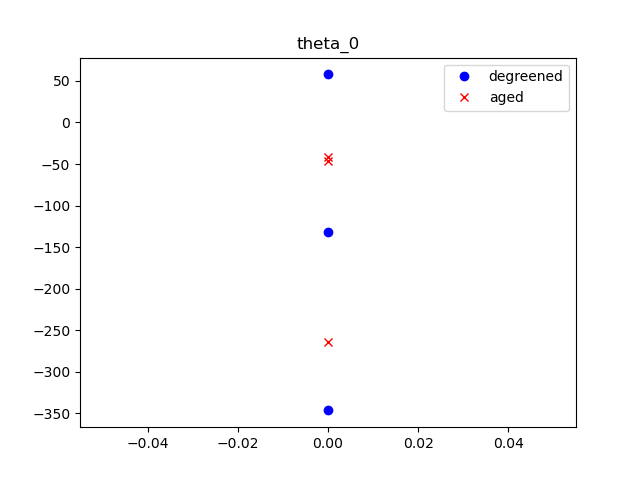
\includegraphics[width = \textwidth]{\froot/figs/figs_new_mdl/theta_0.png}
        \end{minipage}
        \begin{minipage}{0.33\textwidth}
                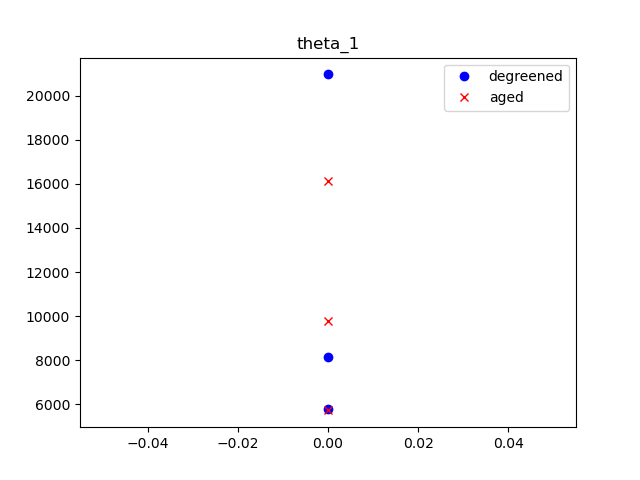
\includegraphics[width = \textwidth]{\froot/figs/figs_new_mdl/theta_1.png}
        \end{minipage}
        \begin{minipage}{0.33\textwidth}
                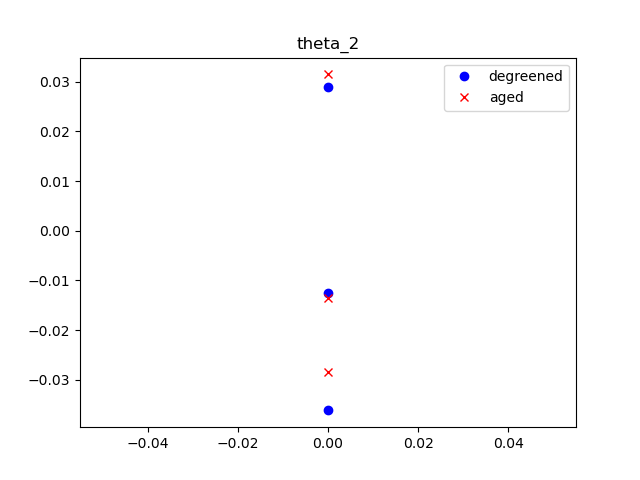
\includegraphics[width = \textwidth]{\froot/figs/figs_new_mdl/theta_2.png}
        \end{minipage}
\end{figure}

\begin{figure}[H]
        \begin{minipage}{0.33\textwidth}
                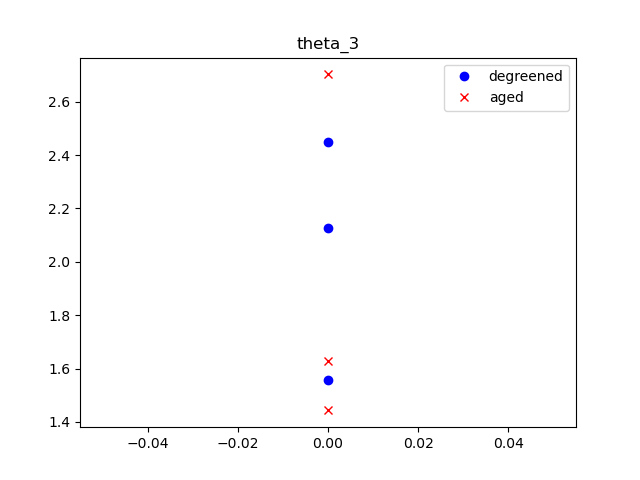
\includegraphics[width = \textwidth]{\froot/figs/figs_new_mdl/theta_3.png}
        \end{minipage}
        \begin{minipage}{0.33\textwidth}
                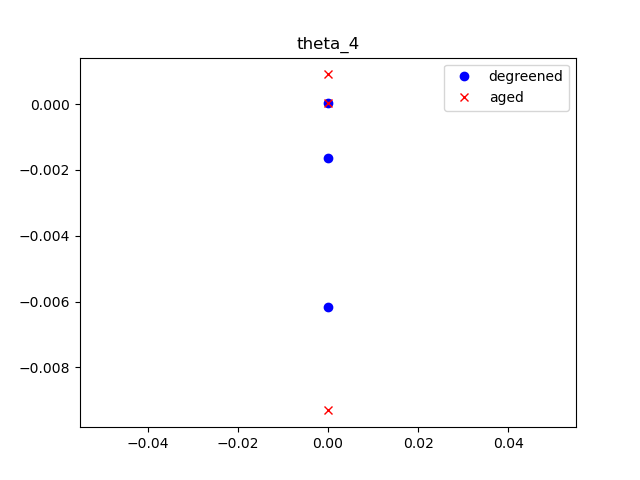
\includegraphics[width = \textwidth]{\froot/figs/figs_new_mdl/theta_4.png}
        \end{minipage}
        \begin{minipage}{0.33\textwidth}
                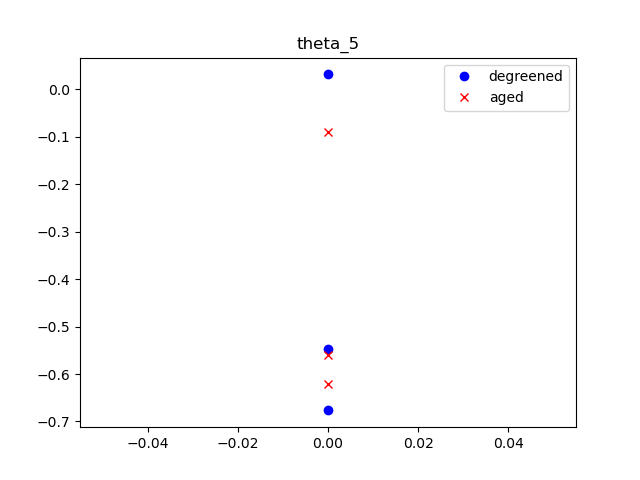
\includegraphics[width = \textwidth]{\froot/figs/figs_new_mdl/theta_5.png}
        \end{minipage}
\end{figure}

\begin{figure}[H]
        \begin{minipage}{0.33\textwidth}
                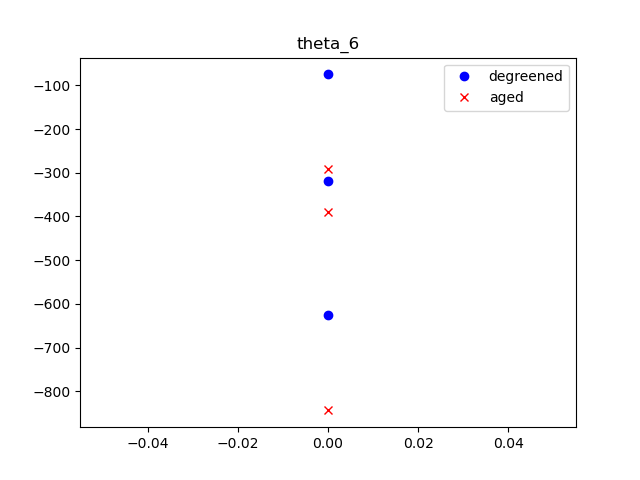
\includegraphics[width = \textwidth]{\froot/figs/figs_new_mdl/theta_6.png}
        \end{minipage}
        \begin{minipage}{0.33\textwidth}
                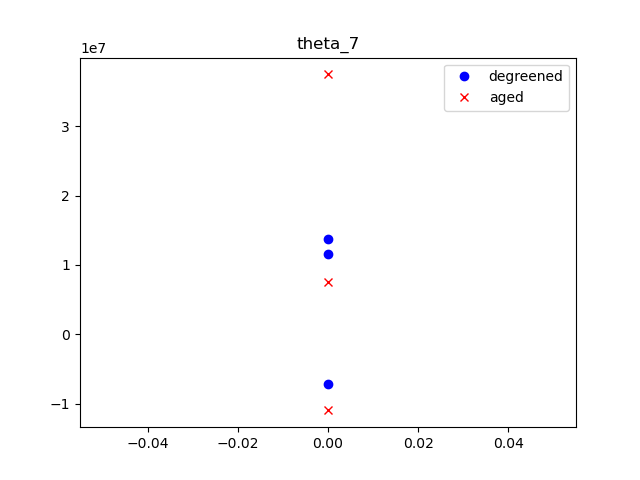
\includegraphics[width = \textwidth]{\froot/figs/figs_new_mdl/theta_7.png}
        \end{minipage}
        \begin{minipage}{0.33\textwidth}
                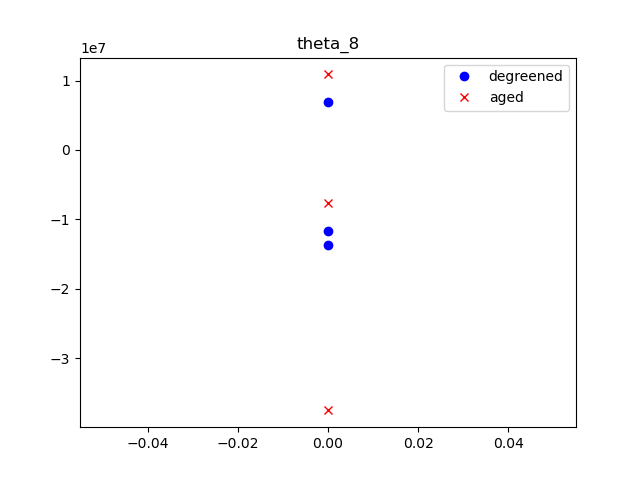
\includegraphics[width = \textwidth]{\froot/figs/figs_new_mdl/theta_8.png}
        \end{minipage}
\end{figure}

\begin{figure}[H]
        \centering
        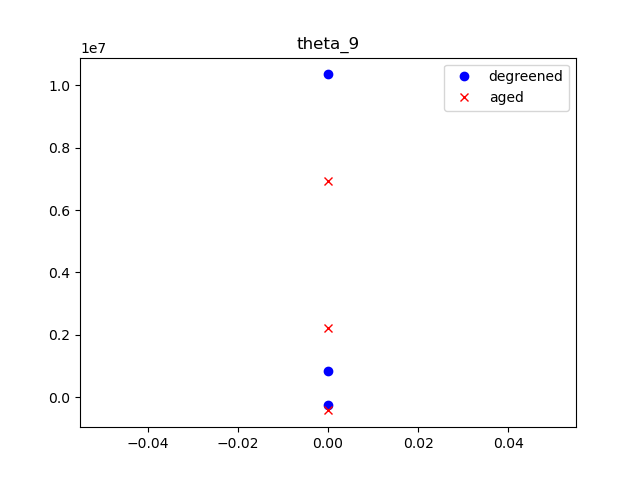
\includegraphics[width = 0.33\textwidth]{\froot/figs/figs_new_mdl/theta_9.png}
\end{figure}

